\documentclass{article}
\usepackage[utf8]{inputenc}
\usepackage[german]{babel}
\usepackage{amsmath}
\usepackage{amsfonts}
\usepackage{amssymb}
\usepackage{graphicx}
\usepackage[left=2cm,right=3cm,top=2cm,bottom=2cm]{geometry}

\title{Pflichtenheft}

\begin{document}

\maketitle
\newpage
\tableofcontents
\newpage

\part{Ausgangssituation und Zielsetzung}
Im Rahmen des Sommersemesterbeleges 2014 im Fach Software Engeneering II der Hochschule für Technik und Wirtschaft Dresden soll ein Softwaresystem zur vereinfachten Erfassung und Verwaltung von Beleggruppen unter Frau Professorin Hauptmann, weiterhin als Auftraggeberin benannt, erstellt werden.
Folgende Aufgabenstellung ist dabei zu realisieren:
Entwickeln  Sie ein SW-System, das die Verwaltung der Daten für Belegarbeiten, die auch parallel laufen können. Neben der Erfassung sind auch weitere Anwendungsfälle wie zum Beispiel „archivieren von Daten“ zu realisieren.
Dazu wird im folgendem die Aufgabenstellung auf 2 Programme aufgeteilt, Eines für die Studenten zum Anmelden und Verwalten ihrer eigenen Gruppe und zum anderen ein Programm für den Dozenten , welcher neben administrativer Funktionen auch Verwaltungsrelevante bekommt.

\newpage 
\part{Systemeinsatz, Systemumgebung}
\subsection{Anwendungsbereiche}
Das System wird zur Verwaltung von Beleggruppen unter dem Auftraggeber eingesetzt. Daher sind einige Festlegungen wie z.B.: die Caseanzahl ausdrücklich vom Auftraggeber festgelegt.
Das System soll als Client-Server Architektur realisiert werden. Der Datenbankserver wird dabei vom Auftraggeber gestellt und unterliegt daher weiterführend keiner genaueren Betrachtung. Zu Implementieren seien daher:
\begin{itemize}
\item Ein Programm damit Studentengruppen eine Gruppe erstellen und verwalten können
\item Ein Programm für den Dozenten mit erweiterten Funktionen hinsichtlich administrativer und verwaltungsrelevanter Aufgaben
\item Verwaltungsstruktur auf dem Datenbankserver um Informationen langfristig zu speichern
\end{itemize}
\subsection{Zielgruppe}
Das Softwaresystem wird zum einen von Studenten benutzt, welche unter dem Auftraggeber eine Belegarbeit anzufertigen haben und sich dazu in Gruppen einfinden und organisieren müssen.
Des Weiteren wird das System vom Auftraggeber sowie von Ihr festgelegten weiteren Berechtigten genutzt werden um die Studenten bei der Verwaltung ihrer Gruppe zu unterstützen sowie selbst eine einfachere Verwaltung von Belegarbeiten zu erhalten.
\subsection{Systemumgebung}
Das Softwaresystem kann nur im Intranet der Hochschule für Technik und Wirtschaft Dresden benutzt werden. 

\newpage
\part{Benutzerschnittstellen}
\section{Client für Studenten}
\begin{center}
    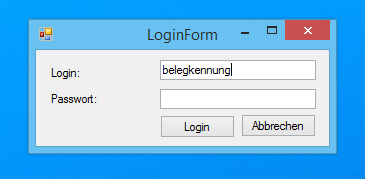
\includegraphics{bilder/pic3.PNG}\\
    Erstanmeldung für Studenten \\
    
    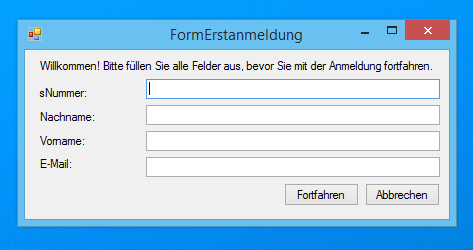
\includegraphics{bilder/pic4.PNG}\\
    Eingabe der persönlichen Informationen des Gruppenleiters \\
    
   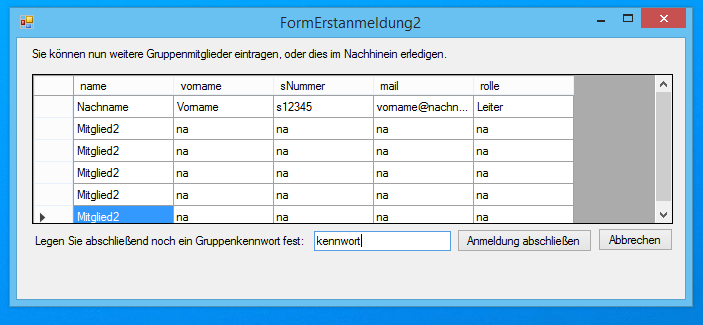
\includegraphics[scale=0.8]{bilder/pic6.PNG}\\
    Gruppenmitglieder werden automatisch in der gegebenen Mindestanzahl erstellt und können bearbeitet werden. Weiter erst nach Eingbabe eines Gruppenpassworts. \\
    
    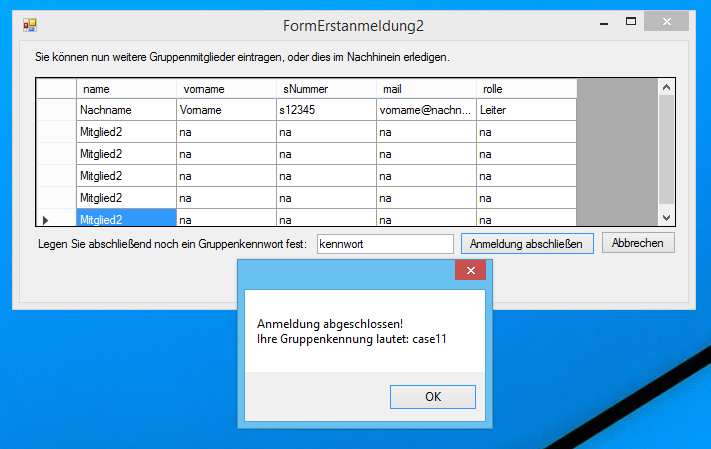
\includegraphics[scale=0.8]{bilder/pic7.PNG}\\
    Ist die Erstanmeldung erfolgreich abgeschlossen, wird vom System eine caseXX-Nummer zugeteilt, die die Gruppe in Zukunft als Gruppen-Login verwendet. \\
    
    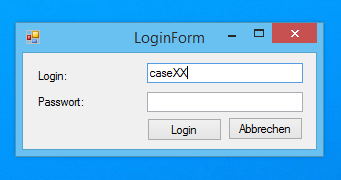
\includegraphics{bilder/pic2.PNG}\\
    Anmeldung für Studenten, wenn schon eine Gruppe existiert \\
\end{center}
\newpage
\section{Client für Dozenten}
\begin{center}
    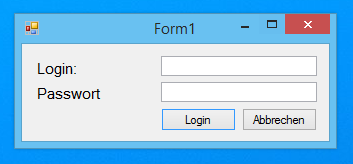
\includegraphics{bilder/doz1.PNG}\\
    Anmeldung für Dozenten \\
    
    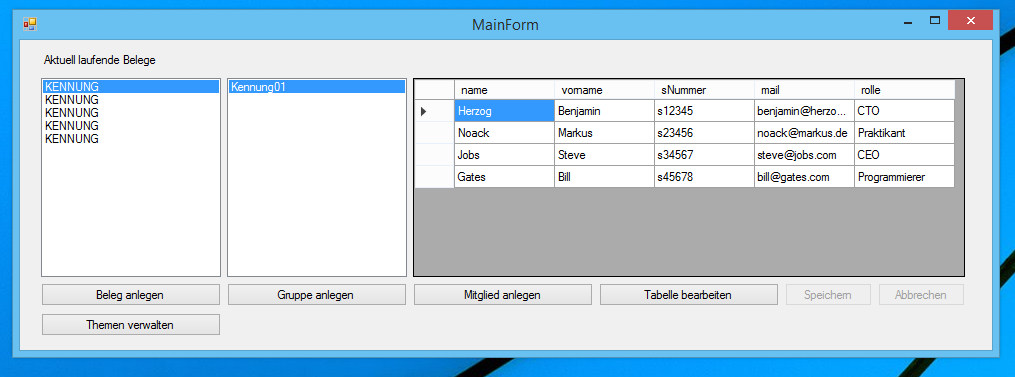
\includegraphics[scale=0.6]{bilder/doz2.PNG}\\
    Übersicht über alle Belege, dessen Gruppen und dessen Mitglieder direkt nach Anmeldung \\
    
    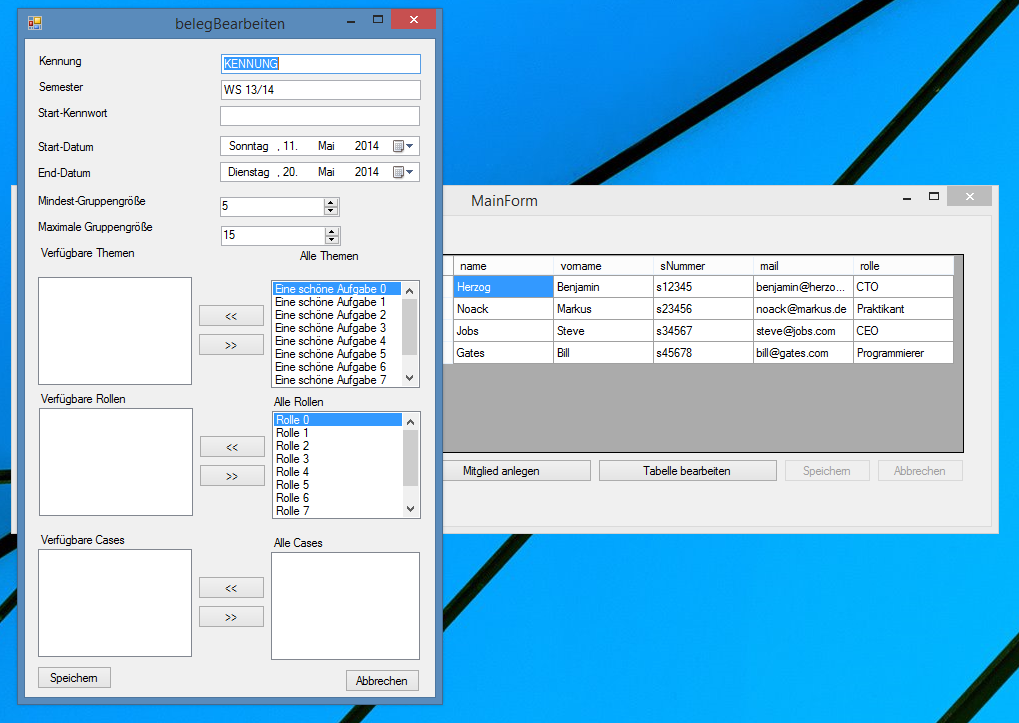
\includegraphics[scale=0.6]{bilder/doz3.PNG}\\
    Anlegen eines neuen Belegs mit den dazugehörigen Angaben \\
    
    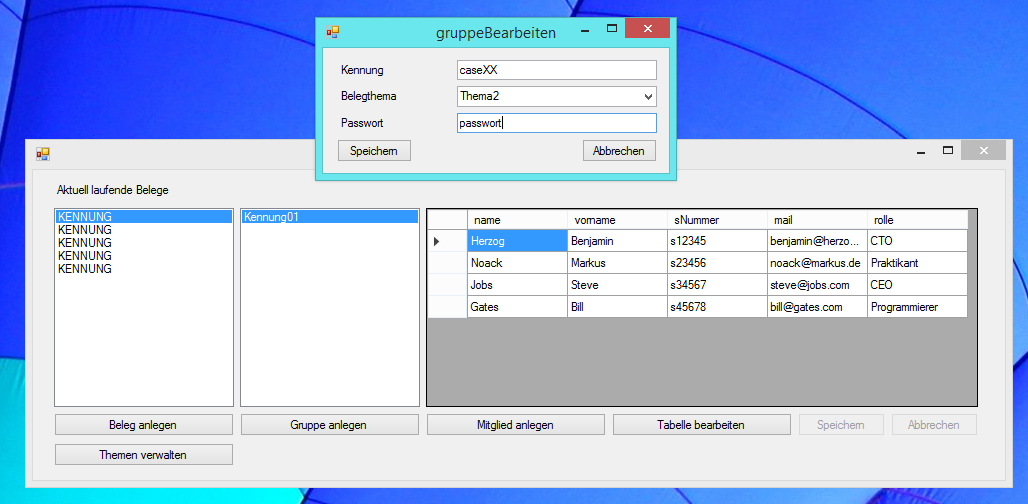
\includegraphics[scale=0.6]{bilder/doz4.PNG}\\
    Gruppe bearbeiten/anlegen, falls Studenten Zugangsdaten oder änhliches vergessen haben \\
    
    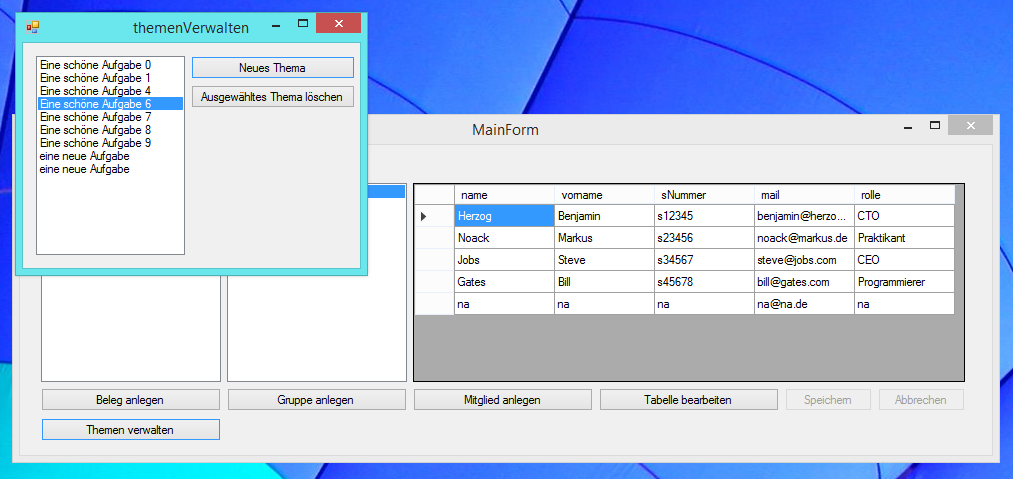
\includegraphics[scale=0.6]{bilder/doz5.PNG}\\
    Themen verwalten (anlegen/löschen) \\
\end{center}



\newpage
\part{Funktionale Anforderungen}
\begin{itemize}
\item Login mit verschiedenen Berechtigungen(Projektgruppe/Dozent)
\item hierarchische Auswahl der Auflistung der Belege, der Gruppen, der Daten
der Gruppenmitglieder für Dozenten
\item Erstellung neuer Belege \& Zuteilung einer Anzahl an Gruppenslots(Cases)
\begin{itemize}
\item Zuteilung von Themen und dem Beleg aus einem bearbeitbaren Themenpool durch Dozent
\item Zuteilung von Rollen und dem Beleg aus einem bearbeitbaren Rollenpool durch Dozent
\end{itemize}
\item lesender/schreibender Zugriff des Dozenten auf sämtliche Daten
\item Generierung einer PDF-Datei mit entsprechenden Daten des Beleges
\item Ausgabe von Datensätzen nach Erfüllung einstellbarer Kriterien(Namen,
Rollenverteilung)
\begin{itemize}
\item relevant für Suchfunktionen und Generierung von E-Mail-Addresslisten
\end{itemize}
\end{itemize}
\begin{itemize}
\item Erstellung neuer Gruppen auf Basis eines vorgegebenen Beleg-Erstlogins
\item tabellarische Auflistung der Gruppendaten aus Gruppenperspektive
\item Änderungsfunktionen der Gruppendaten aus Gruppenperspektive
\end{itemize}

Optional:
\begin{itemize}
\item Thunderbird-Schnittschnelle(direktes öffnen)
\item druckbares Formular zur Benotung
\end{itemize}

\newpage
\part{Qualitätsanforderungen}
\begin{itemize}
\item Benutzerfreundlichkeit (wird über Prototyp geregelt)
\item Zuverlässigkeit (Überprüfung von potentiellen Fehleingaben des Nutzers)
\item Sicherheit und Datenschutz (Gruppen durch Passwort geschützt)
\end{itemize}

\newpage
\part{Rahmenbedingungen}
\begin{itemize}
\item Nutzung des hochschuleigenen Sybase-Servers
\item Die Datenbank (Sybase-DB) zum Speichern der Daten ist bereits vorhanden
(organisatorisch)
\item Anmeldung der Gruppe über einzelnes Login
\item Das Betriebssystem, auf dem das Softwaresystem hauptsächlich lauffähig
sein soll, ist Windows 7(technisch)
\item Gefordert ist eine Desktopanwendung (keine Webanwendung) (technisch)
\item Ein Thema darf von mehreren Gruppen bearbeitet werden (organisatorisch)
\item Beleggruppe darf innerhalb des Anmeldezeitraums flexibel mit Thema und Verantwortlichkeiten (Rollen) umgehen
\item Für das Speichern der Benutzerdaten (z.B. der Email-Adressen) gilt das
Datenschutzgesetz (rechtlich)
\end{itemize}

\newpage
\part{Fehlertoleranzmaßnahmen}

\section{Generell}
\begin{description}
\item[Fehler:] Verbindung Datenbank schlägt Fehl
\item[Reaktion:] Fehlermeldung anzeigen, erneut versuchen oder beenden
\end{description}

\begin{description}
\item[Fehler:] SQL-Injection bei Eingabe von Daten für Datenbankabfragen
\item[Gegenmaßnahme:] Einfügen von Escape-Zeichen vor `'` und `"` oder entfernen selbiger
\end{description}

\section{Gruppe erstellen}
\begin{description}
\item[Fehler:] falsche Zugangsdaten eingegeben
\item[Reaktion:] Fehlermeldung anzeigen, Verzögerung in Datenbank, erneut versuchen
\end{description}
\begin{description}
\item[Fehler:] maximale Gruppenanzahl erreicht
\item[Reaktion:] Fehlermeldung, abbrechen
\end{description}


\newpage
\part{Anforderungen an die Dokumentation}
Was gehört zur Dokumentation?
\begin{itemize}
\item Das Pflichtenheft selbst
\item Entwicklerdokumentation mit Paketdiagramm, Klassendiagrammen, sowie Quellcode-Kommentaren
\item Benutzerdokumentation für Student und Dozent (online als PDF oder schriftlich)
\item Projektdokumentation mit Meilensteinen, Gruppensitzungsprotokollen, Planänderungen und am Ende Reflektion über gesamtes Projekt
\item Testdokumentation mit Testfällen und Testdaten
\end{itemize}

\newpage
\part{Abnahmekriterien}


\newpage
\part{Glossar, Verzeichnisse, Anhang}

\end{document}
